\chapter{Mathematical Expressions} \label{chap:MathExpr}
For many values (boundary conditions, load values) it is possible not
only to prescribe a constant value but also a complex mathematical
expression. CFS++ utilizes for this a customized version of the {\em
  muParser} library (\url{http://muparser.sourceforge.net/}).

\noindent
Therefore one can easily
\begin{itemize}
\item prescribe analytical given, space-dependent, boundary- and load
  conditions, like e.g. a parabolic flow profile or a linear varying load
\item use time and frequency dependent variables to incorporate time-/
  frequency-dependent values
\item generate an analytical time-function, like $sin(\omega t
  + \phi)$ without actually loading it from an external timedata file
  with discrete values
\end{itemize}

\noindent
Currently the following xml-elements allow the prescription of mathematical
expressions:
\begin{itemize}
\item \xel{dirichletInhom} for the \xat{value} and
\xat{phase} attribute
\item \xel{load} for the \xat{value} and \xat{phase}
attribute
\item \xel{regionLoad} in the mechanic PDE for the attribute
\xat{value}
\end{itemize}

\section{Built-in expressions and operators}
{\em muParser} already comes with an extensive set of pre-defined
expressions and and functions (see following two tables).

Note that it is currently not possible to define own variables within
the parser, as otherwise any occurrence of a not explicitly defined
variable would create a new one, initialized with zero.
\begin{table}[ht]
\begin{center}
 \caption{Built-in functions}
 \vspace{0.5cm}  
  \begin{tabular}{lll}
    \toprule
    name & \# of args. & description \\
    \midrule 
    \myverb#sin#     & 1 & sine function \\
    \myverb#cos#     & 1 & cosine function \\
    \myverb#tan#     & 1 & tangens function \\
    \myverb#asin#    & 1 & arcus sine function \\
    \myverb#acos#    & 1 & arcus cosine function \\
    \myverb#atan#    & 1 & arcus tangens function \\
    \myverb#sinh#    & 1 & hyperbolic sine function \\
    \myverb#cosh#    & 1 & hyperbolic cosine \\
    \myverb#tanh#    & 1 & hyperbolic tangens function \\
    \myverb#asinh#   & 1 & hyperbolic arcus sine function \\
    \myverb#acosh#   & 1 & hyperbolic arcus tangens function \\
    \myverb#atanh#   & 1 & hyperbolic arcur tangens function \\
    \myverb#log2#    & 1 & logarithm to the base 2 \\
    \myverb#log10#   & 1 & logarithm to the base 10 \\
    \myverb#log#     & 1 & logarithm to the base 10 \\
    \myverb#ln#      & 1 & logarithm to base e (2.71828...) \\
    \myverb#exp#     & 1 & e raised to the power of x \\
    \myverb#sqrt#    & 1 & square root of a value \\
    \myverb#sign#    & 1 & sign function -1 if $x<0$; 1 if $x>0$ \\
    \myverb#rint#    & 1 & round to nearest integer \\
    \myverb#abs#     & 1 & absolute value \\
    \myverb#if#      & 3 & if ... then ... else ... \\
    \myverb#min#     & var. & min of all arguments \\
    \myverb#max#     & var. & max of all arguments \\
    \myverb#sum#     & var. & sum of all arguments \\
    \myverb#avg#     & var. & mean value of all arguments \\
    \bottomrule
  \end{tabular}
\end{center}
\end{table}

\begin{table}[ht]
\begin{center}
 \caption{Built-in operators and constants}
 \vspace{0.5cm} 
  \begin{tabular}{lll}
    \toprule
    operator & \ meaning & priority \\
    \midrule
    \myverb#=#                  & assignment      & -1 \\
    \myverb#and#                & logical and      & 1 \\
    \myverb#or#                 & logical or       & 1 \\
    \myverb#xor#                & logical xor      & 1 \\
    \myverb#<=# or \verb#le# *  & less or equal    & 2 \\
    \myverb#>=# or \verb#ge# *  & greater or equal & 2 \\
    \myverb#!=#                 & not equal        & 2 \\
    \myverb#==#                 & equal            & 2 \\
    \myverb#># or \verb#gt# *   & greater than     & 2 \\
    \myverb#<# ot \verb#lt# *   & less than        & 2 \\
    \myverb#+#                  & addition         & 3 \\
    \myverb#-#                  & subtraction      & 3 \\
    \myverb#*#                  & multiplication   & 4 \\
    \myverb#/#                  & division         & 4 \\
    \myverb#^#                  & raise x to the power of y & 5 \\
    \myverb#pi#   or \verb#_pi# & $\pi = 3.1415926..$ & \\
    \myverb#_e#                 & Eulerian number $e = 2.7182818..$ \\
 	\bottomrule
  \end{tabular}
\end{center}
  \vspace*{0.5cm}
  {\footnotesize * Due to the restriction in the xml language definition no '$<$' or
    '$>$' signs are allowed in tokens. Therefore the latter form is the
    only one possible in .xml-files. If scripting is used, both forms are
    possible. }
\end{table}
\clearpage
\section{Defining own variables}
%
In addition to the built-in predefined variables, the user can define own
variables within the \xel{variableList}-element of the \xel{domain}-section:
\begin{xmllisting}
<domain>
  <variableList>
    <var name="freq" value="1e6"/>     <!-- excitation frequency -->
    <var name="c"    value="1500"/>    <!-- average speed of sound -->
  </variableList>
  <regionList>
   ...
</domain>
\end{xmllisting}
The registered variables get defined in the global scope and can be used in any
expression, which gets parsed by the mathParser. Note however, that the
variables must evaluate to a constant, i.e. it is NOT allowed to define a
variable like
\begin{xmllisting}
 <!-- NOT ALLOWED -->
 <var name="time" value="5*t"/>
\end{xmllisting}
as this would NOT evaluate to a constant!
%
\section{CFS custom variables}
%
Also CFS++ itself registers some variables related to the current simulation
which can be used in mathematical expressions (see
the following table).
\begin{table}[ht]
\begin{center}
 \caption{CFS specific variables}
 \vspace{0.5cm}
  \begin{tabular}{lp{0.4\textwidth}p{0.4\textwidth}}
    \toprule \rowcolor{darkgrey}
     name & value & occurrence \\
    \midrule
    \xatv{t}     & Current time value       & \xel{transient} analysis \\
    \xatv{dt}    & Time step size $\Delta t$& \xel{transient}
analysis \\
    \xatv{f}     & Current frequency value  & \xel{harmonic} analysis \\
    \xatv{step}  & Current time/frequency step  &
\xel{harmonic},\xel{transient} analysis \\
    \xatv{$x$}, \xatv{$y$}, \xatv{$z$} & Global coordinate of current  node /
element & boundary conditions and loads \\
    \xatv{r}, \xatv{phi}, \xatv{z} & Current local coordinate value & regionLoad
    with cylindrical coordinate system \\
    \bottomrule
  \end{tabular}
\end{center}
\end{table}
%
\clearpage
\section{CFS custom functions}
%
\subsection{\texttt{spike}}
Generates a short spike signal of a given duration (see
Fig. \ref{fig:signalSpike}) starting from 0.
%
\begin{figure}[h!]
 \begin{center}
   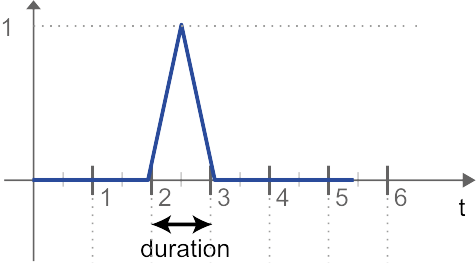
\includegraphics[width=8cm]{pics/sigSpike.png}
 \end{center}
  \caption{Example for spike signal: \xatv{spike(1,t-2)}}
  \label{fig:signalSpike}
\end{figure}
%
\begin{mathFunc}
{spike(duration, timeval)}
 \param{duration} &  Duration of the spike in $s$.\\
 \param{timeval} & Time parameter at which function gets evaluated.
           Usually the time variable \xatv{$t$} is used.
\end{mathFunc}
%
\subsection{\texttt{fadeIn}}
%
This function is used to perform a fadein of an excitation (see Fig.
\ref{fig:signalFade}).
The returned value is between zero and one and has to be
used as envelope of the excitation signal.
%
\begin{figure}[h!]
 \begin{center}
   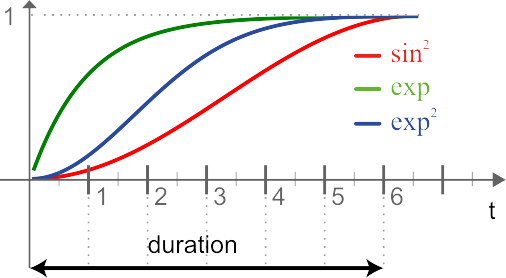
\includegraphics[width=8cm]{pics/sigFade.png}
 \end{center}
  \caption{Comparison of 3 fadeIn signals: $sin^2$-based (red), $exp$-based
(green) and $exp^2$-based (blue).}
  \label{fig:signalFade}
\end{figure}
%
\begin{mathFunc}
{fadeIn(duration, mode, timeval) }
 \param{duration} &  The amount of time for which the fade in
operation is performed in $s$.\\
\param{mode} & Three different implementation exist for
the envelope of the fade in process:
\begin{itemize}
\item 1: using a $sin^2$ formulation
\item 2: using an exponential formulation $exp$
\item 3: using a squared exponential formulation $exp^2$
\end{itemize} \\
\param{timeval} & Time parameter at which function gets evaluated.
           Usually the time variable \xatv{$t$} is used.
\end{mathFunc}
%
\subsection{\texttt{sinBurst}}
%
Creates data for a sine burst signal. A sine burst signal
denotes a sine that will be active during a certain amount
of time until it will be deactivated (see Fig. \ref{fig:signalSinBurst}).
Additionally, a fade-in/out can be applied, according to the $sin^2$ method of
the \texttt{fadeIn} to reduce the higher harmonics of the signal (see Fig.
\ref{fig:signalSinBurstFade}).
\begin{figure}[h!]
 \begin{center}
   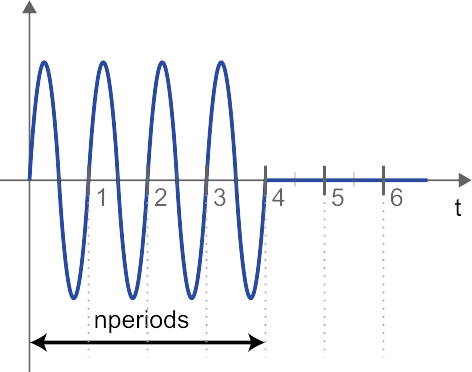
\includegraphics[width=8cm]{pics/sigSinBurst.png}
 \end{center}
  \caption{Sine burst without fade-In: \xatv{sinBurst(1,6,0,0,t)}}
  \label{fig:signalSinBurst}
\end{figure}
\begin{figure}[h!]
 \begin{center}
   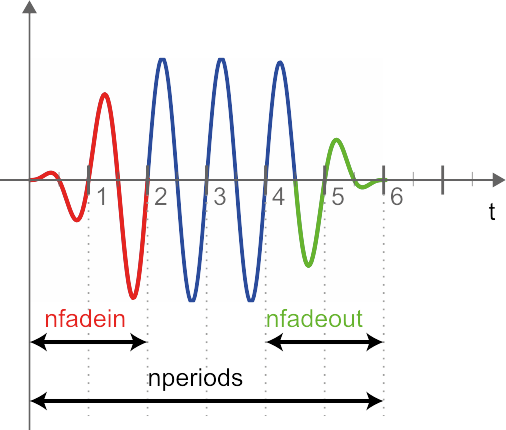
\includegraphics[width=8cm]{pics/sigSinBurstFade.png}
 \end{center}
  \caption{Sine burst with 2 periods of fade-in/out: \xatv{sinBurst(1,6,2,2,t)}}
  \label{fig:signalSinBurstFade}
\end{figure}
\begin{mathFunc}
{sinBurst(freq, nperiods, nfadein, nfadeout, timeval)}
\param{freq} &  Frequency of the sine pulse.\\
\param{nperiods} &  Total number of periods of the pulse.\\
\param{nfadein} &  Specifies the number of periods that will be
used for the transient process. This will realize a kind of "soft" transient
process that will reduce the higher harmonics of the resulting signal.\\
\param{nfadeout} &  Specifies the number of periods that will be
used for the decay process. This will realize a kind of "soft" decay process
that will reduce the higher harmonics of the resulting
signal. \\
\param{timeval} & Time parameter at which function gets evaluated.
           Usually the time variable \xatv{$t$} is used.
\end{mathFunc}
%
\subsection{\texttt{squareBurst}}
%
Create data for a square burst signal, which can either be unipolar or bipolar
(see Fig. \ref{fig:signalSquareBurst} ).
\begin{figure}[h!]
 \begin{center}
   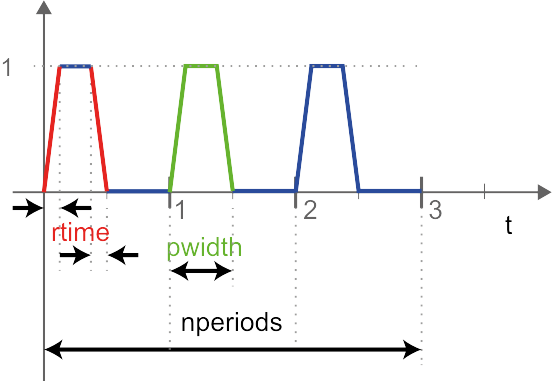
\includegraphics[width=8cm]{pics/sigSquareBurst.png}
 \end{center}
  \caption{Unipolar square burst.}
  \label{fig:signalSquareBurst}
\end{figure}
%
\begin{mathFunc}
{squareBurst(freq, nperdios, bipolar, pwidth, rtime, timeval )}
\param{freq} &  Frequency of the rectangular signal.\\
\param{nperiods} &  Total number of periods of the pulse.\\
\param{bipolar} & Switch for generating bipolar / unipolar signal
\begin{itemize}
 \item 0: unipolar signal ($ 0 \leq y \leq 1$)
 \item 1: bipolar signal ($ -1 \leq y \leq 1$)
\end{itemize} \\
\param{pwidth} & Pulse width of the signal in percent ($0 \leq pw \leq 100$). \\
\param{rtime} & Defines the rise time of the square burst. It denotes the time
                in seconds that the pulse will take to change from low to
                high level. \\
\param{timeval} & Time parameter at which function gets evaluated.
           Usually the time variable \xatv{$t$} is used.
\end{mathFunc}
%
\subsection{\texttt{gauss}}
Generates a Gaussian curve, which is either normalized to a maximum value of 1
or to having an area of 1.
%
\begin{mathFunc}
{gauss(mue, sigma, normval, timeval)}
\param{mue} & Mean value of Gauss curve.\\
\param{sigma} & Variance of Gauss curve.\\
\param{normval} & Type of normalization:
\begin{itemize}
\item 0: Maximum of curve gets normalized to 1
\item 1: Area of curve gets normalized to 1
\end{itemize} \\
\param{timeval} & Time parameter at which function gets evaluated.
           Usually the time variable \xatv{$t$} is used.
\end{mathFunc}

\subsection{\texttt{locCoord2D}}
\label{sec:mathFunc-locCoord2D}
%
This function returns for a point in a 2D cartesian coordinate system one
component of a local coordinate system, as defined in the
\xel{coordSysList}-section of the \xel{domain}-element (for details, see
\ref{sec:coordSys}). This can be used, e.g. to define loads / dirichlet boundary
conditions depending on polar / cylindrical coordinates.
%
\begin{mathFunc}
{locCoord2D(coordsysid, component, x, y)}
\param{coordsysid} & Id string of the referred coordinate system.\\
\param{component} & Coordinate component of the local coordinate system,
which can be either 1 or 2 in 2D. For a polar coordinate system,
1=$r$-direction and 2=$\varphi$-direction.\\
\param{x} & $x$-coordinate of the Cartesian point. For \xel{load} and
\xel{dirichletInhom} boundary conditions, it can be literally replaced by
\xatv{x}. \\
\param{y} & $y$-coordinate of the Cartesian point. For \xel{load} and
\xel{dirichletInhom} boundary conditions, it can be literally replaced by
\xatv{y}.
\end{mathFunc}
In the following example, a cylindrical coordinate system with id \xatv{mid} is
defined. A Dirichlet boundary condition is applied, with a value varying with
the angle $\varphi$ (second component in a polar coordinate system). 
\begin{xmllisting}
<domain>
  <coordSysList>
    <polar id="mid">
      <origin x="0" y="0"/>
      <rAxis x="1" y="0"/>
    </polar>
  </coordSysList>
</domain>
....
<dirichletInhom name=".." value="locCoord('mid',2,x,y)"/>
\end{xmllisting}
%
\subsection{\texttt{locCoord3D}}
%
Similar to the function \texttt{locCoord2D} (see
\ref{sec:mathFunc-locCoord2D}), this method can be used for local 3-dimensional
coordinate systems (e.g. cylindrical or spherical).
%
\begin{mathFunc}
{locCoord3D(coordsysid, component, x, y,z)}
\param{coordsysid} & Id string of the referred coordinate system.\\
\param{component} & Coordinate component of the local coordinate system,
which can be either 1, 2 or in 3D. For a cylindrical coordinate system,
1=$r$-direction, 2=$\varphi$-direction and 3=$z$-direction.\\
\param{x} & $x$-coordinate of the Cartesian point. For \xel{load} and
\xel{dirichletInhom} boundary conditions, it can be literally replaced by
\xatv{x}. \\
\param{y} & $y$-coordinate of the Cartesian point. For \xel{load} and
\xel{dirichletInhom} boundary conditions, it can be literally replaced by
\xatv{y}.\\
\param{z} & $z$-coordinate of the Cartesian point. For \xel{load} and
\xel{dirichletInhom} boundary conditions, it can be literally replaced by
\xatv{z}.
\end{mathFunc}
%
\subsection{\texttt{sample1D}}
This function can be used to read in and interpolate values of a 2-column
formatted text file. This can be used e.g. to prescribe
space/time/frequency-dependent boundary or load conditions.
%
\begin{mathFunc}
{sampled1D(filename, interpolation, sampleval)}
\param{filename} & Name of the file to be read (any path in the filename is
taken relative to the location of the .xml-file). The file must consist of
exactly 2 columns, which are separated by any whitespace (space, tab). \\
\param{interpolation} & There are 3 different methods for interpolating the
sampled values:
\begin{itemize}
 \item 0: Nearest neighbor is taken (i.e. no interpolation at all)
 \item 1: Linear interpolation
 \item 2: Cubic spline interpolation
\end{itemize} \\
\param{sampleval} & Denotes the sample value (value of the 1st column ), for
which a value in the 2nd column is seeked. In most cases either the current
time \xatv{t} or a coordinate component (\xatv{x},\xatv{y}, \xatv{z}) may be
used.
\end{mathFunc}
%
We can subscribe boundary conditions with values read in from sample files.
The notation is as follows:
\begin{xmllisting}
<bcsAndLoads>
  <neumannInhom name="transducer" value="sample1D('x_amplitude.dat',x,2)"
    phase="sample1D('x_phase.dat',x,2)"/>
</bcsAndLoads>
\end{xmllisting}
Sample data (2$^{nd}$ column) is read in from the files x\_amplitude.dat and
x\_phase.dat depending on the current $x$-coordinate and gets interpolated using
cubic spline interpolation. Please note the type of quotes used!!!!
%
\subsection{\texttt{input}}
%
The \texttt{input} function can be used to read in data on a whole region from
HDF5 (or other) files of a previous simulation run. It is used in the
following way:
\begin{xmllisting}
<fileFormats>
  <input>
    <hdf5 fileName="filename.h5" id="inhom"/>
  </input>
  ...
</fileFormats>
...
<pdename>
  <bcsAndLoads>
    <dirichletInhom name="region1" dof="x" value="input('inhom',1,1)"
                    phase="input('inhom',1,1)"/>
    <dirichletInhom name="region2" dof="y" value="input('inhom',1,2)"
                    phase="input('inhom',1,0)"/>
  </bcsAndLoads>
</pdename>
\end{xmllisting}
%
\begin{mathFunc}
{input(fileid, sequencestep, dof)}
\param{fileid} & \xatv{id} of the input file (given under \xel{fileFormats}).\\
\param{sequencestep} & number of the multisequence step (which should be 1 in
  almost any case). \\
\param{dof} & index of the degree of freedom (i.e.\ 1 for \xatv{x}, 2 for
  \xatv{y}, etc.). This argument can be 0, if the degree of freedom should be
  determined automatically (where supported).
\end{mathFunc}
The region name, quantity, and time/frequency step (if applicable) are
determined automatically and not passed as arguments. Therefore it is required
to use exactly the same mesh as the previous simulation, i.e.\
interpolation onto a different mesh is not supported. 

Because some of the information (mentioned above) is determined internally in
\texttt{CFS++}, the \texttt{input} function is currently available only for
some selected boundary conditions, but not all. Table~\ref{tab:input_func}
shows supported boundary conditions.

\begin{table}[h]
  \caption{Boundary conditions supported by the \texttt{input} function}
  \label{tab:input_func}
  \centering
  \begin{tabular}{llp{6cm}}
    \toprule
    \textbf{Boundary condition} & \textbf{Field} & \textbf{Quantity} \\
    \midrule
    \xel{dirichletInhom} & all fields      & the primary unknown, e.g.\ 
        \xatv{mechDisplacement} in mechanics, etc. \\\midrule
    \xel{neumannInhom}   & acoustic        & \xatv{acouVelocity} \\
                         & (potential formulation) & \\\\
                         & acoustic        & \xatv{acouAcceleration} \\
                         & (pressure formulation) & \textbf{Note:} You have to
        multiply \xatv{acouAcceleration} by the density of the acoustic medium
        yourself (e.g.\ \texttt{"1.204*input(...)"} for air), otherwise the
        boundary condition will be incorrect! \\\\
                         & electrostatic   & \xatv{elecCharge} \\\\
                         & heat conduction & \textbf{???} \\\midrule
    \xel{pressure}       & mechanic        & \xatv{mechPressure}, i.e.\
        surface normal stress \\
    \midrule
    \xel{load}           & acoustic        & \xatv{acouRhsLoad} \\
                         & electrostatic   & \xatv{elecRhsLoad}, i.e.\ nodal
                                             charge \\
                         & heat conduction & \xatv{heatRhsLoad} \\
                         & mechanic        & \xatv{mechRhsLoad}, i.e.\ nodal
                                             force \\
    \bottomrule
  \end{tabular}
\end{table}


\section{Examples}
If one wants to prescribe a linear space dependent load, the following can be
written:
\begin{xmllisting}
<bcsAndLoads>
  <load name="loadNode" value="10 * x" phase="cos(y)"/>
<bcsAndLoads>
\end{xmllisting}
Here \myverb#x# is used to denote the x-coordinate of each node
contained in the node list.
\newline

\noindent
To define a variable with a sine of 1 kHz one can simply write:
\begin{xmllisting}
<bcsAndLoads>
  <dirichletInhom name="bcNode" value="10 * sin(2 * pi * 1e3 * t)"/>
<bcsAndLoads>
\end{xmllisting}
The variable \xatv{t} reflects the current time value in a transient
simulation.
Of course one can also combine space- and time dependency:
\begin{xmllisting}
<bcsAndLoads>
  <dirichletInhom name="bcNode" value="10 * x * sin(2 * pi * 1e3 * t)"/>
<bcsAndLoads>
\end{xmllisting}
A ramp signal, which goes from $0 \ldots 1$ linearly and then
stays at 1 is written via the \xatv{if}-statement as follows:
\begin{xmllisting}
<bcsAndLoads>
  <dirichletInhom name="bcNode" value="if(t lt 1,t,1.0)"/>
<bcsAndLoads>
\end{xmllisting}

